\documentclass[11pt]{article}

% ACL format (from Assignment3/format.tex); "final" shows the author names.
\usepackage[final]{acl}
\usepackage{times}
\usepackage{latexsym}
\usepackage[T1]{fontenc}
\usepackage[utf8]{inputenc}
\usepackage{microtype}
\usepackage{inconsolata}
\usepackage{graphicx}
\usepackage{amsmath,amssymb}
\usepackage{booktabs}
\usepackage{xcolor}
\usepackage{enumitem}
\setlist{nosep,leftmargin=*}
\usepackage{tikz}
\usetikzlibrary{arrows.meta,decorations.pathreplacing,calc}
% same palette as the charts (tools/make_figures.py)
\definecolor{cblue}{HTML}{2A78D6}\definecolor{corange}{HTML}{EB6834}\definecolor{caqua}{HTML}{1BAF7A}
\definecolor{inkc}{HTML}{52514E}\definecolor{mutedc}{HTML}{8A8985}
% charts are drawn at their printed size by tools/make_figures.py: include them unscaled
\graphicspath{{../docs/figures/}}
% screenshot: printed only if report/screenshots/<file> exists
\newcommand{\shot}[2]{\IfFileExists{screenshots/#1}{\begin{figure}[h]\centering
  \includegraphics[width=\columnwidth]{screenshots/#1}\caption{#2}\end{figure}}{}}


\title{Merging Consecutive Layers of a Multilingual Language Model:\\
Annealed Absorption and Gradual Layer Flattening on Qwen3}

\author{Sumit Kumar Jha \\
  Roll No.\ 26210180 \\
  IIT Gandhinagar \\
  \texttt{sumitjha@iitgn.ac.in}}

\begin{document}
\maketitle

\begin{abstract}

I try to make Qwen3-0.6B-Base shallower by merging pairs of neighbouring layers instead of deleting them. Between 2
and 8 of its 28 layers are removed (and 4 from Qwen3-1.7B-Base), and every model is tested in six languages (en, hi,
fr, es, de, zh) plus two that are never used for calibration or training (ja, ru). I compare two methods of my own
against plain dropping, a drop + distillation control trained exactly like the methods, and LaCo. The first, AAM,
keeps whichever layer of a pair works better on its own, fades the other one out and distills. The second,
PRISM-Shrink, starts from the exact parallel union of the two layers and shrinks it down to one layer while
distilling. AAM gives the best accuracy: +2.3 points over the control at 4 layers on 0.6B ($p=0.002$), +3.2 on 1.7B,
and the gain is significant on all three seeds. PRISM-Shrink has the smallest perplexity increase once 4 or more
layers are removed (+16.6\,\% against +24.2\,\% for the control, mean of 3 seeds), but it does not improve accuracy.
The gains are modest, though: with 4 or more layers gone from the 0.6B model every method is close to random
guessing, and even AAM keeps only 21\,\% of the original's above-chance skill. If the goal is memory, 8-bit quantization
saves far more at almost no cost.
\end{abstract}

% =====================================================================================================================
\section{Introduction}

A decoder-only transformer runs its $L$ layers one after another, and each layer adds an update to the token's
running state, the residual stream: $h_{i+1} = h_i + f_i(h_i)$. Qwen3-0.6B-Base has $L=28$ such layers
\citep{qwen3}. Every layer that is removed is one sequential step less at inference time. The simplest way to remove
layers is to delete the ones whose input and output are already similar, measured by angular distance
\citep{gromov2024,shortgpt}. But deleting a layer throws away whatever it
wrote into the residual stream, and merging is a way to keep the work of both layers of a pair in one.

I evaluate in several languages because a shared layer has to work for all of them, and a merge that is harmless in
one language may not be in another. I measure damage with perplexity, few-shot accuracy on five benchmarks and an
in-context copying probe.

My contributions are a controlled multilingual comparison (matched control, paired bootstrap tests, three seeds, and
a check that the original model is competent on each test cell), the AAM method together with the observation that
the choice of kept layer is what drives accuracy, and PRISM-Shrink, a gradual and distilled version of layer
flattening \citep{flattengpt} trained on ICL-packed text.

% =====================================================================================================================
\section{Background: from the basics to this work}
\label{sec:background}

\begin{figure*}[t]
\centering
% Decoder-only transformer (top) and one layer with its residual stream (bottom). Full text width.
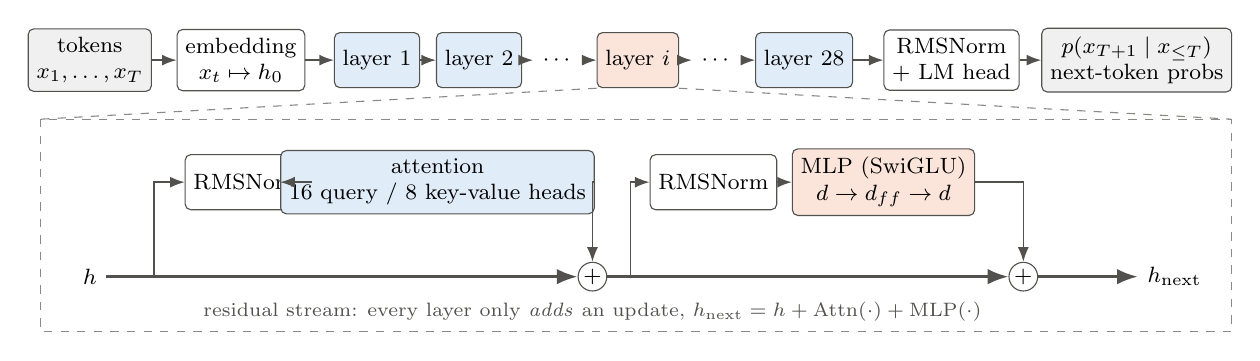
\begin{tikzpicture}[font=\footnotesize, >=Latex, x=0.96cm]
\tikzset{box/.style={draw=inkc, rounded corners=2pt, minimum height=7mm, inner sep=3pt, align=center, fill=white},
         arr/.style={->, draw=inkc, line width=0.5pt}, sum/.style={circle, draw=inkc, inner sep=0.6pt, fill=white}}
\node[box, fill=gray!12] (t) at (0.75,0) {tokens\\$x_1,\dots,x_T$};
\node[box] (e) at (2.75,0) {embedding\\$x_t \mapsto h_0$};
\node[box, fill=cblue!14] (L1) at (4.55,0) {layer 1};
\node[box, fill=cblue!14] (L2) at (5.9,0) {layer 2};
\node (d1) at (6.95,0) {$\cdots$};
\node[box, fill=corange!18] (Li) at (8.0,0) {layer $i$};
\node (d2) at (9.05,0) {$\cdots$};
\node[box, fill=cblue!14] (L28) at (10.2,0) {layer 28};
\node[box] (head) at (12.15,0) {RMSNorm\\+ LM head};
\node[box, fill=gray!12] (p) at (14.6,0) {$p(x_{T+1} \mid x_{\le T})$\\next-token probs};
\foreach \a/\b in {t/e, e/L1, L1/L2, L2/d1, d1/Li, Li/d2, d2/L28, L28/head, head/p} \draw[arr] (\a) -- (\b);
% zoom into layer i
\draw[dashed, draw=mutedc] (0.1,-0.75) rectangle (15.85,-3.45);
\draw[dashed, draw=mutedc] (Li.south west) -- (0.1,-0.75);
\draw[dashed, draw=mutedc] (Li.south east) -- (15.85,-0.75);
\node[sum] (s1) at (7.4,-2.75) {$+$};
\node[sum] (s2) at (13.1,-2.75) {$+$};
\node (hin) at (0.75,-2.75) {$h$};
\node (hout) at (15.1,-2.75) {$h_{\mathrm{next}}$};
\draw[arr, line width=1pt] (hin) -- (s1);
\draw[arr, line width=1pt] (s1) -- (s2);
\draw[arr, line width=1pt] (s2) -- (hout);
\node[box] (n1) at (2.85,-1.55) {RMSNorm};
\node[box, fill=cblue!14] (att) at (5.35,-1.55) {attention\\16 query / 8 key-value heads};
\node[box] (n2) at (9.0,-1.55) {RMSNorm};
\node[box, fill=corange!18] (mlp) at (11.25,-1.55) {MLP (SwiGLU)\\$d \rightarrow d_{ff} \rightarrow d$};
\draw[arr] (1.6,-2.75) |- (n1);
\draw[arr] (n1) -- (att);
\draw[arr] (att) -| (s1);
\draw[arr] (7.9,-2.75) |- (n2);
\draw[arr] (n2) -- (mlp);
\draw[arr] (mlp) -| (s2);
\node[text=inkc, font=\scriptsize] at (7.4,-3.2) {residual stream: every layer only \emph{adds} an update, $h_{\mathrm{next}} = h + \mathrm{Attn}(\cdot) + \mathrm{MLP}(\cdot)$};
\end{tikzpicture}

\caption{Top: a decoder-only language model turns tokens into vectors, refines them through 28 layers and predicts
the next token. Bottom: inside one layer, attention and the MLP each read a normalised copy of the state and
\emph{add} their output to the residual stream.}
\label{fig:transformer}
\end{figure*}

Text is split into tokens (Qwen3 has a vocabulary of 151{,}936), and an embedding table turns each token into a
vector of size $d$, which is 1{,}024 for the 0.6B model. The model predicts $p(x_t \mid x_{<t})$ and is trained with
the cross-entropy $-\frac{1}{T}\sum_t \log p(x_t \mid x_{<t})$. The exponential of this loss is the perplexity, and
lower is better.

Figure~\ref{fig:transformer} shows one transformer layer, which computes
\begin{align}
N(x) &= \gamma \odot x \,/\, \sqrt{\tfrac{1}{d}\textstyle\sum_j x_j^2 + \epsilon}, \\
h' &= h + \mathrm{Attn}\big(N(h)\big), \\
h_{\mathrm{next}} &= h' + \mathrm{MLP}\big(N(h')\big), \\
\mathrm{Attn}(x) &= \mathrm{softmax}\big(QK^{\top}/\sqrt{d_h} + M\big)\,V, \\
\mathrm{MLP}(x) &= W_{d}\big(\mathrm{SiLU}(W_{g}x) \odot W_{u}x\big),
\end{align}
where $N$ is RMSNorm, $Q, K, V$ are linear maps of $x$, $M$ is the causal mask, and $W_g, W_u, W_d$ are the gate,
up and down projections; grouped-query attention shares each key-value head between 2 of the 16 query heads.

Since each layer only adds an update to $h$, the residual stream changes slowly. In the middle of the network the
updates are small and neighbouring layers see almost the same input (cosine 0.96--0.97); merging neighbours relies
on this.

In few-shot prompting the prompt contains solved examples, and a base model answers
by continuing the pattern. This depends on \emph{induction heads}, attention heads that find an earlier copy of the
current token and predict the token that followed it \citep{olsson2022}. Knowledge distillation \citep{hinton2015}
trains a smaller or damaged student to match the teacher's output distribution (through a KL divergence) rather than
only the correct token. Layer pruning deletes the layers whose input and output are most similar
\citep{gromov2024,shortgpt}, and the deleted layer's contribution is gone unless some other part of the model learns
it. For the statistics I use the bootstrap, which resamples the test questions to get a confidence interval, and a
paired test, which compares two models on the same questions \citep{efron1993}.

\begin{table*}[t]
\centering\small
\begin{tabular}{p{0.18\textwidth}p{0.75\textwidth}}
\toprule
Term & Meaning in this report \\
\midrule
Token, embedding & a piece of text; its vector of size $d$ \\
Layer & one transformer block (attention + MLP); Qwen3-0.6B and 1.7B have 28 \\
Residual stream & the running state $h$ of a token; each layer adds its update to it \\
Attention head, KV group & one attention pattern; a key-value head with the 2 query heads that share it \\
MLP neuron & one of the $d_{ff}$ hidden units of the feed-forward block \\
Perplexity & $\exp$ of the average next-token loss; how unsure the model is (lower is better) \\
Few-shot accuracy & share of correct answers when the prompt contains solved examples \\
Random guessing (chance) & 25\,\% on 4-option tests, 33.3\,\% on XNLI, 0\,\% on MGSM; 21.7\,\% on the average \\
Skill kept & share of the original's above-chance accuracy that survives (0 = guessing, 100 = original) \\
Copying loss & loss on the second copy of a repeated random sequence; tests induction heads \\
Distillation (KD) & training a student to match a teacher's next-token distribution \\
Angular distance & angle between the state entering and leaving a pair; small = the pair changes little \\
Drop & delete one layer of each pair, no training \\
Control & drop + the same distillation as the methods (isolates the method's own effect) \\
AAM & keep the better layer of each pair, fade the other out, distill \\
PRISM-Shrink & run the pair as one wide parallel layer, shrink it gradually to one layer, distill \\
Bootstrap CI, paired $p$ & range that contains the result 95\,\% of the time; chance of a difference this large if none existed \\
\bottomrule
\end{tabular}
\caption{Terms used in this report.}
\label{tab:glossary}
\end{table*}

% =====================================================================================================================
\section{Report}

\subsection{Feedback and novelties discussed with the mentor}


This is what I have done since Presentation 2 (the repository history has the details). I first ran a small test of
15 merging algorithms, covering closed-form least squares, gradual distillation, search, the PRISM family and LaCo,
with 100 questions per benchmark and language. I then moved to a large test with 200--250 questions per benchmark
and language, more than 100k unique test tokens per language, per-question results so that bootstrap confidence
intervals can be computed, and Japanese and Russian added as unseen languages. To separate what a method does from
what the training alone does, I added a matched control (drop plus the same distillation). On top of that come a
depth study (2, 4, 6 and 8 layers removed), a second model size (Qwen3-1.7B), a data ablation (kept layer $\times$
training text), a training-length ablation (400 vs 1{,}000 steps) and three seeds.

The new ideas I tried were PRISM (the exact parallel form of a layer pair), PRISM-Shrink (shrinking it gradually),
AAM, ICL-packed training text, CoPlan pair selection, a language-specific residual (LSR), smeared-key merging (SKM)
and a cross-term correction (XTC). SKM, XTC and LSR did not help, and I report them as negative results.

\subsection{Baselines and state of the art}

\begin{table*}[t]
\centering\small
\resizebox{\textwidth}{!}{%
\begin{tabular}{lllll}
\toprule
Method & Idea & Training & Code & Used here \\
\midrule
Drop / ShortGPT \citep{shortgpt,gromov2024} & delete the most similar layers & none & simple & yes (\texttt{drop}) \\
LaCo \citep{laco} & add other layers' weight differences to one layer & none & re-implemented & yes (small test) \\
Layer parallelism \citep{truedepth} & run two layers side by side & optional & public (GitHub) & idea only \\
LLM-Streamline \citep{streamline} & train a small module to replace removed layers & yes & not checked & no \\
FuseGPT \citep{fusegpt} & fold removed blocks into neighbours & yes & not checked & no \\
FlattenGPT \citep{flattengpt} & one wide layer from two, pruned back in one step & optional & not released & closest prior work \\
\midrule
Control (ours) & drop + the same distillation as the methods & yes & this repo & yes \\
\bottomrule
\end{tabular}}
\caption{Baselines and related depth-compression methods.}
\label{tab:baselines}
\end{table*}

The closest earlier work to PRISM-Shrink is FlattenGPT \citep{flattengpt}. It merges two adjacent blocks into one
wider block and then prunes it back to the original width in a single step, without training, and reports
87--96\,\% of zero-shot performance retained at about 20\,\% compression on 7B--70B English models. In my
version the hand-over is gradual and distilled and starts from the exact original pair, the training text is
ICL-packed, and the evaluation is multilingual with a matched control and several seeds.

The control is the baseline I care most about, because it gets the same training as the methods; any gain over it
comes from the method and not from the extra training.

\subsection{Datasets}

\begin{table}[t]
\centering\small
\resizebox{\columnwidth}{!}{%
\begin{tabular}{lll}
\toprule
Use & Data & Size per language \\
\midrule
Calibration & Wiki-40B train \citep{wiki40b} & 16 $\times$ 256 tokens \\
Distillation & Wiki-40B train & 300 $\times$ 256 tokens \\
Perplexity test & mC4 \citep{mt5}, Wiki-40B test & 128 $\times$ 256 each \\
Knowledge & MMMLU \citep{mmmlu,mmlu} & 200 (5-shot) \\
Regional exams & INCLUDE \citep{include} & 200 (5-shot) \\
Maths & MGSM \citep{mgsm} & 250 (4-shot CoT) \\
Reading & Belebele \citep{belebele} & 200 (3-shot) \\
Inference & XNLI \citep{xnli} & 200 (3-shot) \\
\bottomrule
\end{tabular}}
\caption{Data. Tests are never used for fitting or choosing anything. MGSM has no Hindi; INCLUDE has no English.}
\label{tab:data}
\end{table}

Every language gets the same amount of calibration text, and every training step contains one sequence from each
language. Calibration and training only use the Wiki-40B \emph{train} split, and the
pairs to merge are fixed by angular distance on calibration text before anything is tested, so nothing leaks from
the test sets. One calibration sequence per language is held out to measure every fit. A test cell (benchmark
$\times$ language) only counts if the original model is clearly above chance on it; the only flagged cell is German
XNLI on 0.6B. Japanese and Russian are only ever evaluated and never used for anything else, so that damage outside
the training languages shows up. All models get the same shots and prompts, and the shots never overlap with test
items.

The main bottlenecks were GPU time (Kaggle T4s with a weekly quota) and GPU memory: the double-width layer in fp32
ran out of memory at 6 or more layers and on 1.7B. Hindi also needs 2--4$\times$ more tokens per item, and MMMLU has
no development split, so I use its first shuffled rows as shots.

The data grew from the small test (100 questions per benchmark and language) to the large test, with 200--250
questions, 128 instead of 16 perplexity sequences, per-question results, and ja and ru added. That gives more than
100k unique test tokens per language (Table~\ref{tab:tokens} in the appendix). I also built ICL-packed training text.
Each sequence is $[a,\,b,\,a]$: a passage, a passage in another language, and the first passage again (768 tokens in
total), so during training the model has to copy from its own context.

\subsection{Experimental plan}

\subsubsection{Setting, training and robustness}

I choose pairs by the angular distance $d(i) = \frac{1}{\pi}\arccos\cos(h_i, h_{i+2})$ averaged over tokens
\citep{gromov2024}, and never touch the first or last two layers. For Qwen3-0.6B this gives pairs 12-13 and 14-15
when 2 layers are removed and 10-11, 12-13, 14-15 and 16-17 for 4; removing 6 adds 7-8 and 24-25, and removing 8
adds 5-6 and 22-23.

All trained methods share one distillation setup \citep{hinton2015}. The original model is a frozen teacher, and
only the merged layers are trained, with the loss
\begin{align}
\mathcal{L} &= \mathcal{L}_{\mathrm{KL}} + \mathcal{L}_{h}, \\
\mathcal{L}_{\mathrm{KL}} &= \tfrac{1}{T}\textstyle\sum_t \mathrm{KL}\big(p^{\mathrm{tea}}_t \,\|\, p^{\mathrm{stu}}_t\big), \\
\mathcal{L}_{h} &= \lVert h^{s}-h^{t}\rVert^2 / \lVert h^{t}\rVert^2 ,
\end{align}
where $p_t$ is the next-token distribution at position $t$ and $h^{s}, h^{t}$ are the student's and teacher's
hidden states at the output of each merged pair. The part being removed is faded out with
\begin{equation}
\alpha(s) = \tfrac{1}{2}\big(1+\cos(\pi (s+1)/A)\big)
\end{equation}
at step $s$, where $A = 0.7\times 400 = 280$; for the last 120 of the 400 steps $\alpha=0$
(Figure~\ref{fig:alpha}). At $\alpha=1$ the student is exactly the original model, which I checked before training.

\begin{figure}[t]
\centering
% Knowledge distillation used by every trained method. Column width.
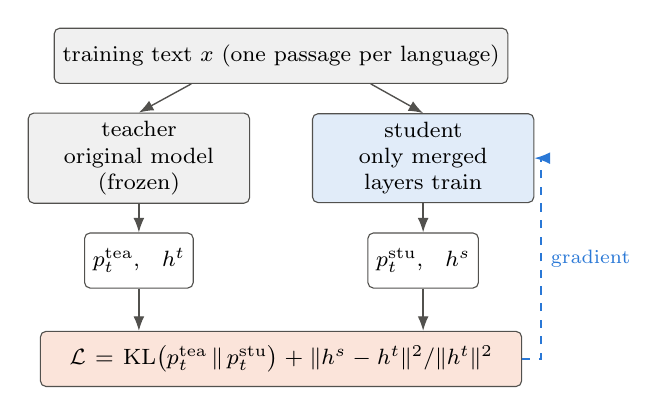
\begin{tikzpicture}[font=\footnotesize, >=Latex, x=0.95cm]
\tikzset{box/.style={draw=inkc, rounded corners=2pt, minimum height=7mm, inner sep=3pt, align=center, fill=white},
         arr/.style={->, draw=inkc, line width=0.5pt}}
\node[box, fill=gray!12] (x) at (3.5,0) {training text $x$ (one passage per language)};
\node[box, fill=gray!12, text width=2.6cm] (T) at (1.6,-1.3) {teacher\\original model\\(frozen)};
\node[box, fill=cblue!14, text width=2.6cm] (S) at (5.4,-1.3) {student\\only merged layers train};
\node[box] (pt) at (1.6,-2.6) {$p^{\mathrm{tea}}_t$, \; $h^{t}$};
\node[box] (ps) at (5.4,-2.6) {$p^{\mathrm{stu}}_t$, \; $h^{s}$};
\node[box, fill=corange!18, text width=5.9cm] (L) at (3.5,-3.85)
  {$\mathcal{L} = \mathrm{KL}\big(p^{\mathrm{tea}}_t \,\|\, p^{\mathrm{stu}}_t\big) + \lVert h^{s}-h^{t}\rVert^2 / \lVert h^{t}\rVert^2$};
\draw[arr] (x.south) ++(-1.2,0) -- (T.north);
\draw[arr] (x.south) ++(1.2,0) -- (S.north);
\draw[arr] (T) -- (pt); \draw[arr] (S) -- (ps);
\draw[arr] (pt) -- (pt |- L.north); \draw[arr] (ps) -- (ps |- L.north);
\draw[->, dashed, draw=cblue, line width=0.6pt] (L.east) -- ++(0.25,0) |- (S.east) node[pos=0.25, right, font=\scriptsize, text=cblue] {gradient};
\end{tikzpicture}

\caption{Knowledge distillation shared by the control, AAM and PRISM-Shrink: only the merged layers receive gradients.}
\label{fig:distill}
\end{figure}

To keep the comparison fair, every method uses the same pairs, data, shots and training recipe. Beyond that there is
the matched control, paired bootstrap tests on the same questions \citep{efron1993}, three seeds for the main
4-layer runs, the competence check, and two model sizes.

\subsubsection{Models and approaches}

\begin{figure*}[t]
\centering
% The four ways to treat one pair of consecutive layers (A, B). Full text width.
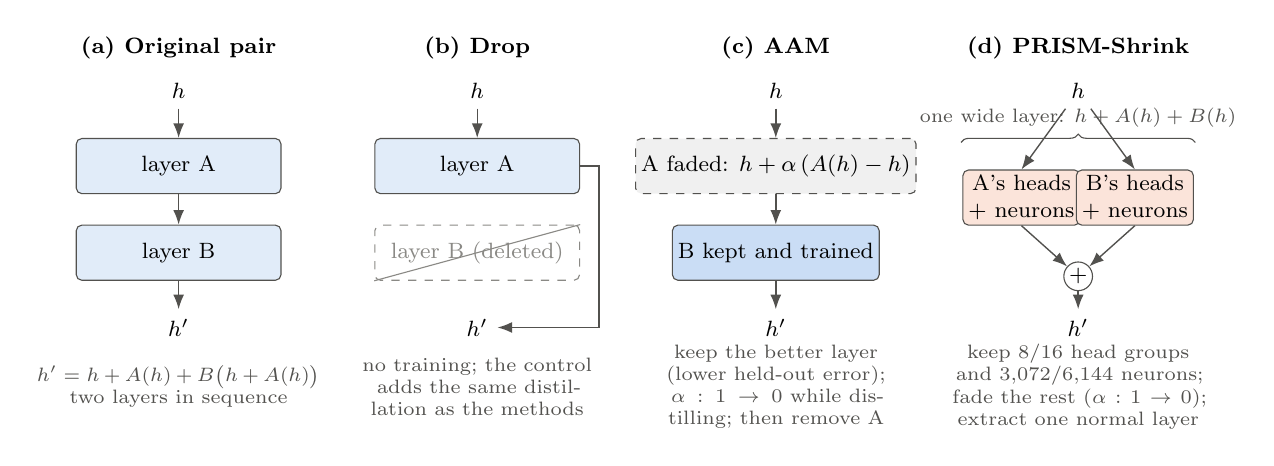
\begin{tikzpicture}[font=\footnotesize, >=Latex, x=0.96cm]
\tikzset{box/.style={draw=inkc, rounded corners=2pt, minimum height=7mm, minimum width=2.6cm, inner sep=2pt, align=center, fill=white},
         arr/.style={->, draw=inkc, line width=0.5pt}, sum/.style={circle, draw=inkc, inner sep=0.6pt, fill=white},
         note/.style={text width=3.6cm, align=center, font=\scriptsize, text=inkc}, ttl/.style={font=\footnotesize\bfseries}}
% (a) original
\node[ttl] at (1.95,0.55) {(a) Original pair};
\node (i1) at (1.95,0) {$h$};
\node[box, fill=cblue!14] (a1) at (1.95,-0.95) {layer A};
\node[box, fill=cblue!14] (b1) at (1.95,-2.05) {layer B};
\node (o1) at (1.95,-3.0) {$h'$};
\draw[arr] (i1) -- (a1); \draw[arr] (a1) -- (b1); \draw[arr] (b1) -- (o1);
\node[note] at (1.95,-3.75) {$h' = h + A(h) + B\big(h + A(h)\big)$\\two layers in sequence};
% (b) drop
\node[ttl] at (5.9,0.55) {(b) Drop};
\node (i2) at (5.9,0) {$h$};
\node[box, fill=cblue!14] (a2) at (5.9,-0.95) {layer A};
\node[box, draw=mutedc, text=mutedc, dashed] (b2) at (5.9,-2.05) {layer B (deleted)};
\draw[draw=mutedc] (b2.south west) -- (b2.north east);
\node (o2) at (5.9,-3.0) {$h'$};
\draw[arr] (i2) -- (a2);
\draw[arr] (a2.east) -- ++(0.25,0) |- (o2.east);
\node[note] at (5.9,-3.75) {no training; the control adds the same distillation as the methods};
% (c) AAM
\node[ttl] at (9.85,0.55) {(c) AAM};
\node (i3) at (9.85,0) {$h$};
\node[box, fill=gray!12, dashed] (a3) at (9.85,-0.95) {A faded: $h + \alpha\,(A(h)-h)$};
\node[box, fill=cblue!25] (b3) at (9.85,-2.05) {B kept and trained};
\node (o3) at (9.85,-3.0) {$h'$};
\draw[arr] (i3) -- (a3); \draw[arr] (a3) -- (b3); \draw[arr] (b3) -- (o3);
\node[note] at (9.85,-3.75) {keep the better layer (lower held-out error); $\alpha: 1 \rightarrow 0$ while distilling; then remove A};
% (d) PRISM-Shrink
\node[ttl] at (13.85,0.55) {(d) PRISM-Shrink};
\node (i4) at (13.85,0) {$h$};
\node[box, minimum width=1.45cm, fill=corange!18] (a4) at (13.1,-1.35) {A's heads\\+ neurons};
\node[box, minimum width=1.45cm, fill=corange!18] (b4) at (14.6,-1.35) {B's heads\\+ neurons};
\node[sum] (s4) at (13.85,-2.35) {$+$};
\node (o4) at (13.85,-3.0) {$h'$};
\draw[arr] (i4) -- (a4.north); \draw[arr] (i4) -- (b4.north);
\draw[arr] (a4.south) -- (s4); \draw[arr] (b4.south) -- (s4); \draw[arr] (s4) -- (o4);
\draw[decorate, decoration={brace, amplitude=3pt}, draw=inkc] (12.3,-0.65) -- (15.4,-0.65)
  node[midway, above=2pt, font=\scriptsize, text=inkc] {one wide layer: $h + A(h) + B(h)$};
\node[note] at (13.85,-3.75) {keep 8/16 head groups and 3{,}072/6{,}144 neurons; fade the rest ($\alpha: 1 \rightarrow 0$); extract one normal layer};
\end{tikzpicture}

\caption{The four ways one pair of consecutive layers (A, B) is treated. Every final model has one standard layer per
pair; AAM and PRISM-Shrink differ in what the remaining layer learns from.}
\label{fig:methods}
\end{figure*}

\textbf{Drop} deletes the second layer of each pair, with no training. The \textbf{control} drops in the same way
and then runs the shared distillation, so the first layer of each pair is kept and trained.

\textbf{AAM} keeps the layer with the lower held-out error when it is used alone. For pair 14-15, for example, the
errors are 28.9\,\% and 26.6\,\%, so L15 is kept. The other layer becomes $h + \alpha(f(h)-h)$, is faded out during
distillation, and is then removed.

\textbf{PRISM} starts from the observation that in the middle of the network
$h + A(h) + B(h + A(h)) \approx h + A(h) + B(h)$, because the inputs of the two layers have cosine 0.96--0.97. The
right-hand side is exactly one wider layer: the attention head groups and MLP neurons of A and B sit side by side,
and each layer's RMSNorm gain is folded into its own input weights. This rewrite is exact; I checked it to
$<10^{-4}$ relative error.

\textbf{PRISM-Shrink} keeps 8 of the 16 key-value head groups and 3{,}072 of the 6{,}144 neurons, chosen by write
energy. The output is $\alpha\,B(A(h)) + (1-\alpha)\,U_\alpha(h)$, where $U_\alpha$ is the wide layer with every
dropped part scaled by $\alpha$. After distillation the kept parts are extracted as a normal layer.

\textbf{LaCo} sets $\theta = \theta_A + \sum_{j\neq A}(\theta_j - \theta_A)$ for every weight and needs no data.

The control and AAM run the same code and differ in a single switch, namely which layer of the pair is kept. The gap
between AAM and the control therefore measures the layer choice, and the gap between PRISM-Shrink and the control
measures merging against deleting. Data, pairs, loss, optimizer and number of steps are the same for all of them.

\subsubsection{Parameters and architecture}

One decoder layer with hidden size $d$, $n_q$ query heads, $n_{kv}$ key-value heads of size $d_h$ and MLP width
$d_{ff}$ has
\begin{equation}
P_{\text{layer}} = 2\,d\,n_q d_h + 2\,d\,n_{kv} d_h + 3\,d\,d_{ff} + 2d + 2d_h ,
\end{equation}
and the model has $P = V d + L\,P_{\text{layer}} + d$ (tied embeddings, vocabulary $V=151{,}936$).

\begin{table}[t]
\centering\small
\begin{tabular}{lrr}
\toprule
 & Qwen3-0.6B & Qwen3-1.7B \\
\midrule
$d$ / $d_{ff}$ & 1{,}024 / 3{,}072 & 2{,}048 / 6{,}144 \\
$n_q$ / $n_{kv}$ / $d_h$ & 16 / 8 / 128 & 16 / 8 / 128 \\
Layers $L$ & 28 & 28 \\
$P_{\text{layer}}$ & 15{,}730{,}944 & 50{,}336{,}000 \\
Embedding $Vd$ & 155{,}582{,}464 & 311{,}164{,}928 \\
Total $P$ & 596{,}049{,}920 & 1{,}720{,}574{,}976 \\
One layer & 2.64\,\% & 2.93\,\% \\
\midrule
4 layers removed & 533{,}126{,}144 & 1{,}519{,}230{,}976 \\
Parameters cut & 10.6\,\% & 11.7\,\% \\
\bottomrule
\end{tabular}
\caption{Parameter counts (checked against the saved results). 2 / 6 / 8 layers removed from 0.6B: 5.3 / 15.8 /
21.1\,\%.}
\label{tab:params}
\end{table}

Every final model is an ordinary Qwen3 model with fewer layers of the same shape, so the architectures only differ
during training. There, PRISM-Shrink holds a double-width layer for each pair (16 head groups, 6{,}144 neurons, plus
a per-head q/k gain table of 5{,}632 parameters), while AAM and the control hold the two original layers with a fade
between them.

\subsubsection{Hyperparameters and ablations}

\begin{table}[t]
\centering\small
\resizebox{\columnwidth}{!}{%
\begin{tabular}{ll}
\toprule
Setting & Value \\
\midrule
Optimizer & AdamW, lr $5\times10^{-5}$, no weight decay \\
Gradient clipping & 1.0 \\
Steps & 400 (1{,}000 in the ablation) \\
Fade schedule & cosine over 280 steps, then 120 at 0 \\
Batch per step & 6 $\times$ 256 tokens (ICL: 6 $\times$ 768) \\
Loss & KL + 1.0 $\times$ hidden MSE \\
Precision & fp16 autocast (1.7B teacher in fp16) \\
Micro-batch & 1{,}536 tokens (512 / 256 when memory-bound) \\
Calibration & 16 $\times$ 256 tokens per language \\
Kept parts (Shrink) & 8/16 head groups, 3{,}072/6{,}144 neurons \\
Seeds & 0 (all runs); 1, 2 (main 4-layer runs) \\
\bottomrule
\end{tabular}}
\caption{Training settings, identical for every trained method.}
\label{tab:hparams}
\end{table}

\begin{table}[t]
\centering\small
\begin{tabular}{lllrrr}
\toprule
Kept layer & Text & Steps & Acc & PPL & Copy \\
\midrule
first (control) & plain & 400 & 23.3 & +25.2 & 0.579 \\
first (control) & ICL & 400 & 23.5 & +24.5 & 0.372 \\
better (AAM) & plain & 400 & \textbf{25.8} & +22.8 & 0.337 \\
better (AAM) & ICL & 400 & 25.1 & +21.6 & \textbf{0.246} \\
better (AAM) & plain & 1000 & \textbf{26.6} & +20.6 & 0.513 \\
union (Shrink) & plain & 400 & 24.3 & +17.5 & 0.218 \\
union (Shrink) & ICL & 400 & 23.5 & \textbf{+16.5} & \textbf{0.212} \\
union (Shrink) & plain & 1000 & 24.0 & \textbf{+15.8} & 0.339 \\
\bottomrule
\end{tabular}
\caption{Ablations, Qwen3-0.6B, 4 layers removed. Acc = few-shot average accuracy (\%), PPL = mC4 perplexity
increase (\%), Copy = copying loss (lower is better).}
\label{tab:ablation}
\end{table}

I did not run a grid search. One Kaggle session per setting costs 1--3.5 GPU hours, so I fixed the recipe (learning
rate, loss weight, fade length 0.7) on the small test and kept it identical for all methods. This keeps the
comparison fair, but it also means no method was tuned for itself. In the ablations, the choice of kept layer moves
accuracy by +1.6 to +2.5 points, while the training text moves it by at most 0.8. Training for 1{,}000 steps lowers
perplexity by about 2 points and changes accuracy by at most +0.8 ($p=0.05$, AAM), but copying gets worse
(Table~\ref{tab:ablation}, Figure~\ref{fig:ablations}).

\subsubsection{Metrics}

For general language-modelling damage I use perplexity,
$\exp\big(-\frac{1}{T}\sum_t \log p(x_t\mid x_{<t})\big)$, on mC4 and Wiki-40B, reported as the increase over the
original model averaged over languages. For task ability I use few-shot accuracy on MMMLU, INCLUDE, MGSM, Belebele
and XNLI, averaged over the five. Random guessing gives 25, 25, 0, 25 and 33.3\,\% on these, which is 21.7\,\% on the
average. I also report the skill kept above chance,
$\frac{1}{5}\sum_b \frac{a_b - c_b}{a^{\text{orig}}_b - c_b}$, and a copying probe in which 32 random 128-token
sequences are shown twice and the NLL is measured on the repeat; this targets induction heads \citep{olsson2022}.
The remaining numbers are accuracy on the unseen languages, prefill and decode speed, and 95\,\% bootstrap confidence
intervals with paired $p$-values.

\subsubsection{System effort and demo scenario}

The large-test queue logged 21.0 session-hours of Kaggle GPU time over 13 paired sessions, three of which failed and
had to be re-run (Table~\ref{tab:gpu} in the appendix). Earlier runs are not in this log. Each session uses two T4
GPUs, with one notebook per GPU.

Demo for the viva. A full 0.6B run takes 1--1.5 hours, so the demo has two parts. Live: run the CPU smoke-test
version of a notebook (\texttt{tools/make\_notebooks.py} builds it with tiny settings: 64-token sequences, a few
training and test items), which goes through every stage (pair selection, AAM or PRISM-Shrink build, distillation,
perplexity, benchmarks, copying probe) in minutes and without a GPU. Then load one compressed model and generate text
from a prompt next to the original model. Saved: open the logged Kaggle runs and rebuild the tables and figures of
this report from their JSON results with \texttt{tools/analyze.py} and \texttt{make\_figures.py}.

\subsection{Project management}

Most of the new ideas came out of analysis or earlier failures. A layer analysis (angular change per layer, write
sizes, update similarity, attention-head roles; Figure~\ref{fig:layers}) showed that the middle layers barely change
the state and read nearly the same input, and that is where the parallel form (PRISM) came from. Closed-form fits
did not hold up on few-shot accuracy, which pushed me towards gradual distillation (AAM, PRISM-Shrink). The copying
probe and the head analysis led to ICL packing.

\begin{table}[t]
\centering\small
\resizebox{\columnwidth}{!}{%
\begin{tabular}{ll}
\toprule
Resource & Used \\
\midrule
GPU & Kaggle, 2 $\times$ NVIDIA T4 (15 GB each) \\
CPU / RAM & Kaggle T4 session: 4 cores, 29 GB \\
Disk & Kaggle working directory, 20 GB (results $<$ 1 GB) \\
Orchestration & local laptop (Kaggle API) \\
GPU time & 21.0 session-hours logged \\
\bottomrule
\end{tabular}}
\caption{Computational resources.}
\label{tab:compute}
\end{table}


% =====================================================================================================================
\section{Experiment}

\subsection{Implementation}
\label{sec:impl}

\begin{figure*}[t]
\centering
% End-to-end experimental pipeline. Full text width.
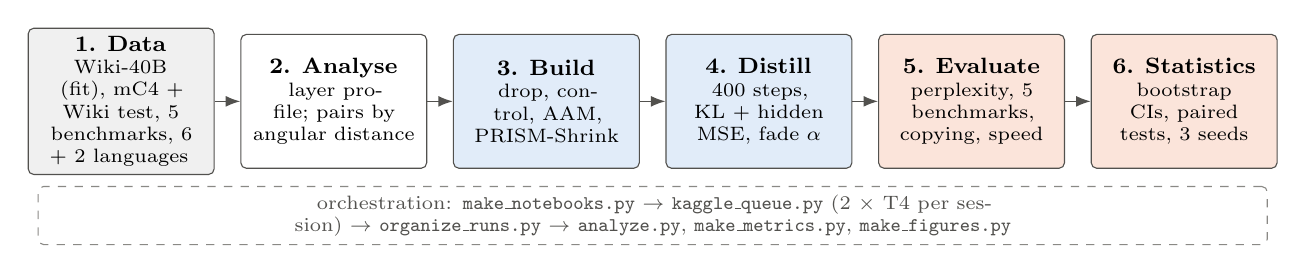
\begin{tikzpicture}[font=\scriptsize, >=Latex]
\tikzset{box/.style={draw=inkc, rounded corners=2pt, minimum height=17mm, text width=2.15cm, inner sep=3pt, align=center, fill=white},
         arr/.style={->, draw=inkc, line width=0.5pt}, hd/.style={font=\footnotesize\bfseries}}
\node[box, fill=gray!12] (d) at (1.2,0) {{\footnotesize\bfseries 1. Data}\\Wiki-40B (fit), mC4 + Wiki test, 5 benchmarks, 6 + 2 languages};
\node[box] (a) at (3.9,0) {{\footnotesize\bfseries 2. Analyse}\\layer profile; pairs by angular distance};
\node[box, fill=cblue!14] (b) at (6.6,0) {{\footnotesize\bfseries 3. Build}\\drop, control, AAM, PRISM-Shrink};
\node[box, fill=cblue!14] (k) at (9.3,0) {{\footnotesize\bfseries 4. Distill}\\400 steps, KL + hidden MSE, fade $\alpha$};
\node[box, fill=corange!18] (v) at (12.0,0) {{\footnotesize\bfseries 5. Evaluate}\\perplexity, 5 benchmarks, copying, speed};
\node[box, fill=corange!18] (s) at (14.7,0) {{\footnotesize\bfseries 6. Statistics}\\bootstrap CIs, paired tests, 3 seeds};
\foreach \a/\b in {d/a, a/b, b/k, k/v, v/s} \draw[arr] (\a) -- (\b);
\node[draw=mutedc, dashed, rounded corners=2pt, text width=15.4cm, align=center, inner sep=3pt, text=inkc] at (7.95,-1.45)
  {orchestration: \texttt{make\_notebooks.py} $\rightarrow$ \texttt{kaggle\_queue.py} (2 $\times$ T4 per session) $\rightarrow$
   \texttt{organize\_runs.py} $\rightarrow$ \texttt{analyze.py}, \texttt{make\_metrics.py}, \texttt{make\_figures.py}};
\end{tikzpicture}

\caption{The end-to-end pipeline, from data to statistics, and the scripts that run it on Kaggle.}
\label{fig:pipeline}
\end{figure*}

The code is at \url{https://github.com/sumitjhaa/gpt2-layermerging} (branch \texttt{assignment3-top3}, folder
\texttt{Assignment3/Sumit}). The pipeline (Figure~\ref{fig:pipeline}) runs in five steps.
\begin{enumerate}
  \item Download and cache Wiki-40B, mC4 and the five benchmarks, and build the calibration, training and test
        splits. A reference run shares these with all other notebooks.
  \item Analyse the layers and choose the pairs by angular distance.
  \item Build the method (\texttt{keep\_one\_build} for AAM and the control, \texttt{shrink\_build} for
        PRISM-Shrink) and distill it.
  \item Evaluate perplexity, the five benchmarks, the copying probe and speed, and write one JSON row per model that
        holds every question's result.
  \item Generate one notebook per experiment (\texttt{tools/make\_notebooks.py}), run them on Kaggle
        (\texttt{tools/kaggle\_queue.py}), file the runs (\texttt{tools/organize\_runs.py}), and rebuild all
        tables and figures (\texttt{tools/analyze.py}, \texttt{make\_metrics.py}, \texttt{make\_figures.py}).
\end{enumerate}

\subsection{Results and findings}

\begin{table*}[t]
\centering\small
\begin{tabular}{llrrrrr}
\toprule
Removed & Method & Acc (\%) & vs drop [95\% CI] & Skill kept & mC4 PPL & Copy \\
\midrule
0 & original & 48.9 & -- & 100\,\% & -- & 0.125 \\
\midrule
2 & drop & 28.7 & -- & 32\,\% & +14.2\,\% & 0.320 \\
2 & control & 29.3 & +0.6 [$-$0.3, +1.5] & 35\,\% & +7.9\,\% & 0.172 \\
2 & AAM & \textbf{34.1} & \textbf{+5.4} [+3.9, +6.8] & \textbf{53\,\%} & \textbf{+6.0\,\%} & 0.203 \\
2 & PRISM-Shrink + ICL & 28.2 & $-$0.4 [$-$1.5, +0.6] & 31\,\% & +6.2\,\% & \textbf{0.131} \\
\midrule
4 & drop & 22.6 & -- & 7\,\% & +84.7\,\% & 2.220 \\
4 & control & 23.5 & +1.0 [$-$0.0, +1.9] & 13\,\% & +24.5\,\% & 0.372 \\
4 & AAM & \textbf{25.8} & \textbf{+3.3} [+1.9, +4.6] & \textbf{21\,\%} & +22.8\,\% & 0.337 \\
4 & PRISM-Shrink + ICL & 23.5 & +0.9 [$-$0.3, +2.3] & 11\,\% & \textbf{+16.5\,\%} & \textbf{0.212} \\
\midrule
6 & drop & 21.5 & -- & 1\,\% & +236.6\,\% & 4.292 \\
6 & control & 22.3 & +0.8 [$-$0.3, +2.0] & 4\,\% & +59.2\,\% & 0.506 \\
6 & AAM & \textbf{23.8} & \textbf{+2.3} [+1.0, +3.7] & \textbf{12\,\%} & +54.7\,\% & 0.519 \\
6 & PRISM-Shrink + ICL & 23.1 & +1.6 [+0.4, +2.8] & 7\,\% & \textbf{+39.4\,\%} & \textbf{0.340} \\
\midrule
8 & drop & 20.9 & -- & $-$2\,\% & +689.4\,\% & 10.112 \\
8 & control & 21.6 & +0.7 [$-$0.4, +1.9] & 1\,\% & +103.8\,\% & 1.091 \\
8 & AAM & \textbf{23.4} & \textbf{+2.5} [+1.1, +4.0] & \textbf{10\,\%} & +103.1\,\% & 0.766 \\
8 & PRISM-Shrink + ICL & 22.3 & +1.4 [+0.3, +2.5] & 4\,\% & \textbf{+69.0\,\%} & \textbf{0.651} \\
\bottomrule
\end{tabular}
\caption{Qwen3-0.6B-Base. Acc = few-shot average accuracy (random guessing 21.7\,\%); vs drop = paired difference
on the same questions; skill kept = share of the original's above-chance accuracy; PPL = mean mC4 perplexity
increase; Copy = copying loss.}
\label{tab:main}
\end{table*}

\begin{table}[t]
\centering\small
\begin{tabular}{lrrrr}
\toprule
Method & Acc & vs drop & PPL & Copy \\
\midrule
original & 58.9 & -- & -- & 0.106 \\
drop & 24.1 & -- & +70.5 & 2.831 \\
control & 30.9 & +6.8 & +32.1 & 1.150 \\
AAM & \textbf{34.1} & \textbf{+10.0} & +29.4 & 0.450 \\
PRISM-Shrink & 31.5 & +7.4 & \textbf{+22.3} & \textbf{0.257} \\
\bottomrule
\end{tabular}
\caption{Qwen3-1.7B-Base, 4 layers removed (all methods trained on plain text). All differences vs drop
$p<0.001$.}
\label{tab:17b}
\end{table}

\begin{table}[t]
\centering\small
\resizebox{\columnwidth}{!}{%
\begin{tabular}{lccc}
\toprule
Method & Acc (seeds 0/1/2) & Mean & vs control \\
\midrule
AAM & 25.8 / 25.4 / 26.1 & 25.8$\pm$0.3 & +1.8 to +2.6$^{*}$ \\
PRISM-Shrink & 23.5 / 23.7 / 23.5 & 23.6$\pm$0.1 & $-$0.0 to +0.1 \\
control & 23.5 / 23.6 / 23.5 & 23.6$\pm$0.1 & -- \\
\bottomrule
\end{tabular}}
\caption{Three seeds, Qwen3-0.6B, 4 layers removed. $^{*}$significant on every seed ($p\le 0.009$). Mean mC4
perplexity increase: AAM +23.0\,\%, PRISM-Shrink +16.6\,\%, control +24.2\,\%.}
\label{tab:seeds}
\end{table}

With plain dropping, perplexity rises by 14\,\% at 2 layers and by 689\,\% at 8, and accuracy is already at chance
from 4 layers on (Table~\ref{tab:main}, Figure~\ref{fig:depth}). Distillation repairs much of this. At 4 layers the
control brings the perplexity increase down from +84.7\,\% to +24.5\,\%, but its accuracy goes up by only 1.0 point
($p=0.05$); on 1.7B the gain is larger, +6.8.

AAM beats the control by +4.8, +2.3, +1.5 and +1.8 points at 2, 4, 6 and 8 layers (all $p\le 0.018$) and by +3.2 on
1.7B (Figure~\ref{fig:forest}). Since AAM and the control differ only in which layer is kept, this gain comes from
the layer choice; with the training text held fixed it is worth +1.6 to +2.5 points (Table~\ref{tab:ablation}).
Over three seeds AAM gets 25.8$\pm$0.3 (Table~\ref{tab:seeds}, Figure~\ref{fig:seedsfig}).

PRISM-Shrink behaves differently. From 4 layers on, its perplexity is lower than both the control's and AAM's in all
6 languages, on mC4 and on Wikipedia, at every depth and on both models (Figure~\ref{fig:lang}), and its copying loss
is the lowest as well. Its accuracy, however, is never significantly different from the control's ($-1.0$ to $+1.0$,
$p\ge 0.07$), so merging helps language modelling but not the benchmarks (Figure~\ref{fig:tradeoff}).

Model size matters a lot here: at 4 layers removed AAM keeps 41\,\% of the above-chance skill on 1.7B and only
21\,\% on 0.6B (Table~\ref{tab:17b}, Figure~\ref{fig:chance}). Maths goes first. MGSM falls from 41\,\% to about
2\,\% for every method at 4 layers (Table~\ref{tab:bench}), and on Belebele drop and the control even end up below
chance (about 20\,\%).

For saving memory, quantization is the better tool. 8-bit quantization halves memory with almost no loss on Qwen3,
and 4-bit loses about 5 MMLU points on Qwen3-8B \citep{qwen3quant}, whereas removing 4 layers here saves 11\,\% and
costs 23 points. In my view layer removal only makes sense for speed (roughly 10--20\,\% faster at 4 layers in my
runs), and it can be combined with quantization.

\begin{figure*}[t]
\centering
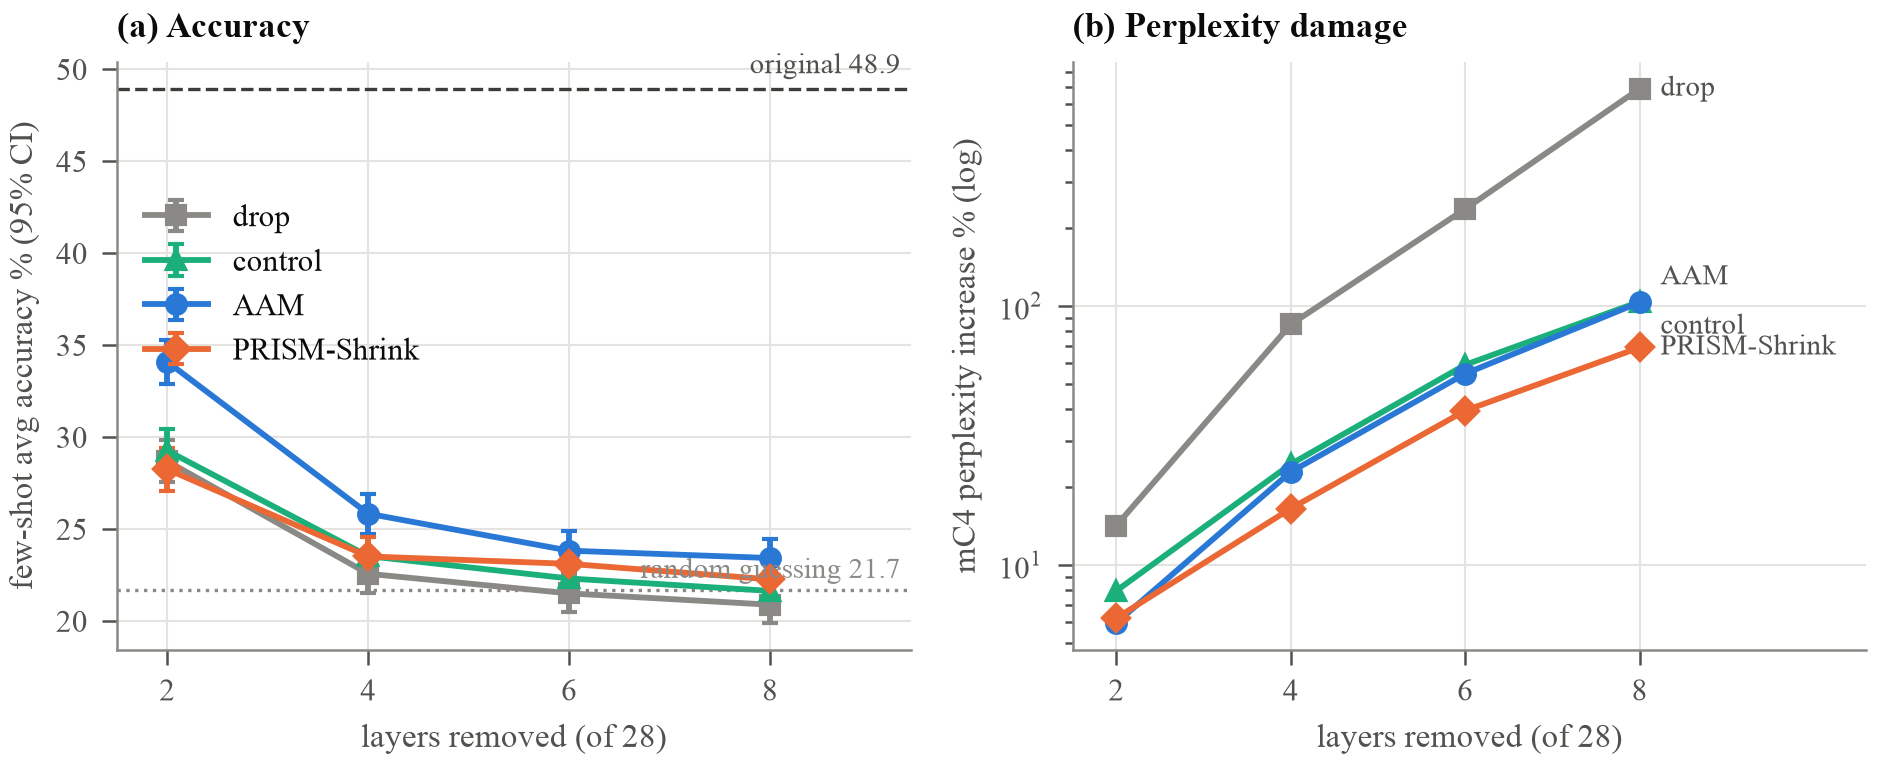
\includegraphics{depth.png}
\caption{Accuracy (95\% CI) and perplexity damage versus layers removed, Qwen3-0.6B.}
\label{fig:depth}
\end{figure*}

\begin{figure*}[t]
\centering
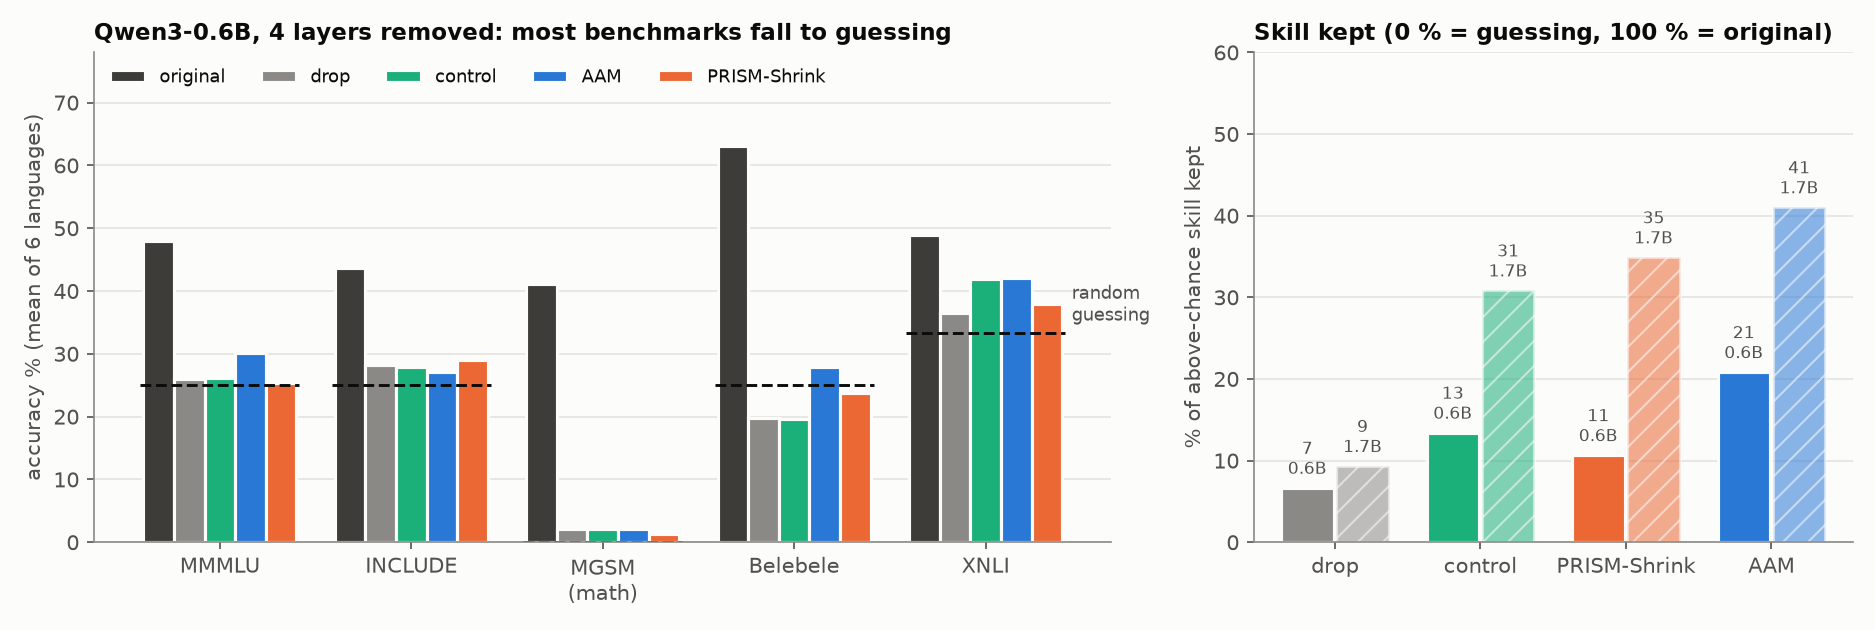
\includegraphics{benchmarks_vs_chance.png}
\caption{Left: each benchmark at 4 layers removed against random guessing (dashed). Right: share of the original's
above-chance skill kept, 0.6B and 1.7B.}
\label{fig:chance}
\end{figure*}

\begin{figure*}[t]
\centering
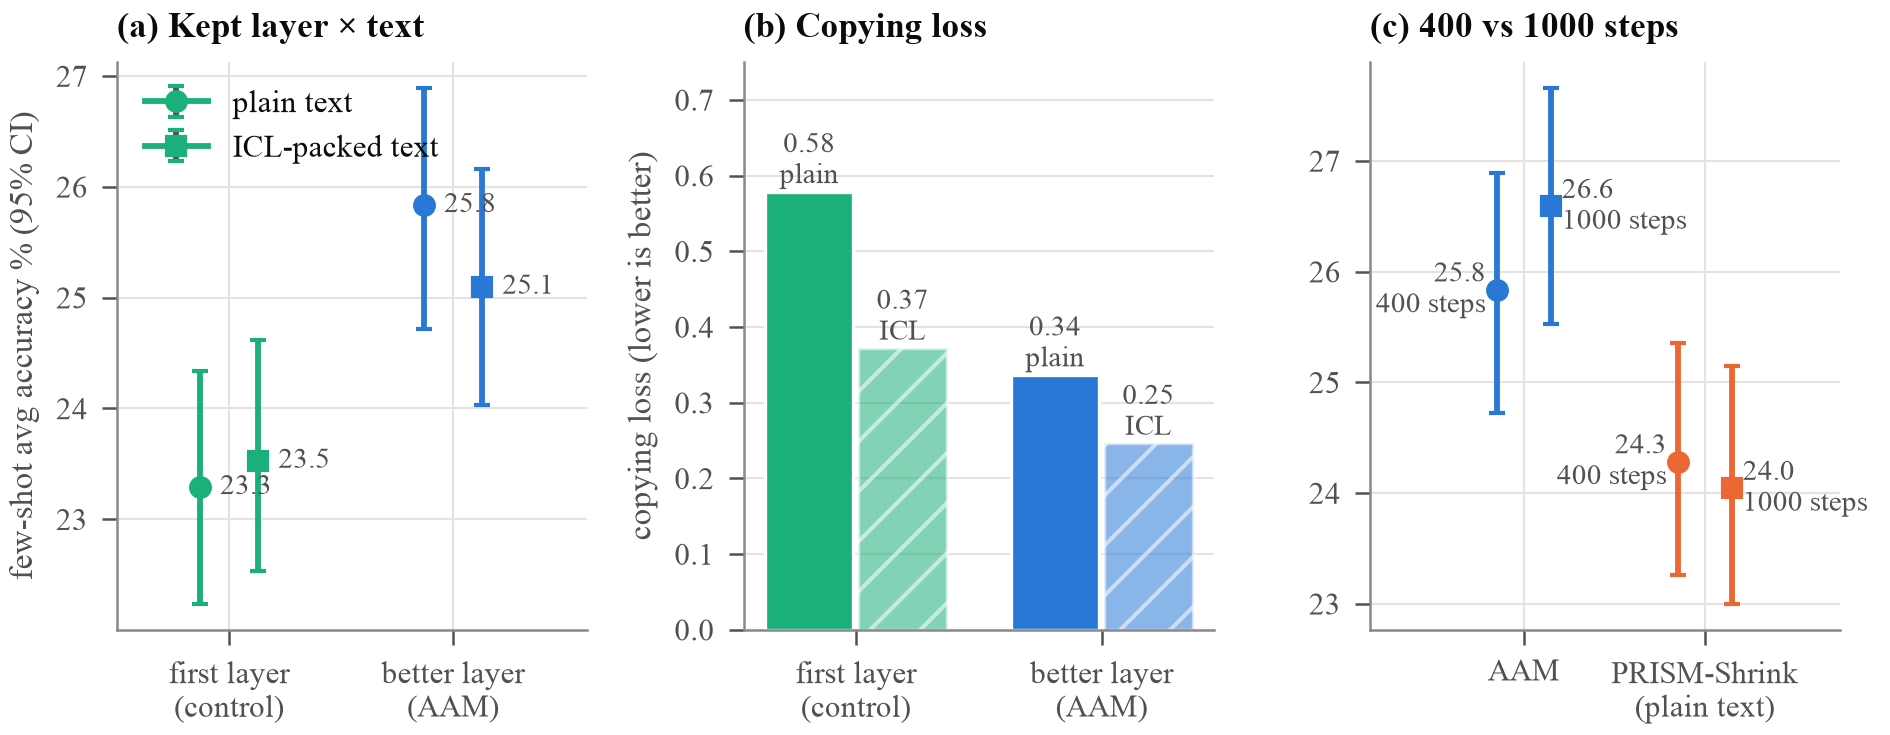
\includegraphics{ablations.png}
\caption{Ablations at 4 layers removed: kept layer $\times$ training text, copying loss, and training length.}
\label{fig:ablations}
\end{figure*}

\begin{figure*}[t]
\centering
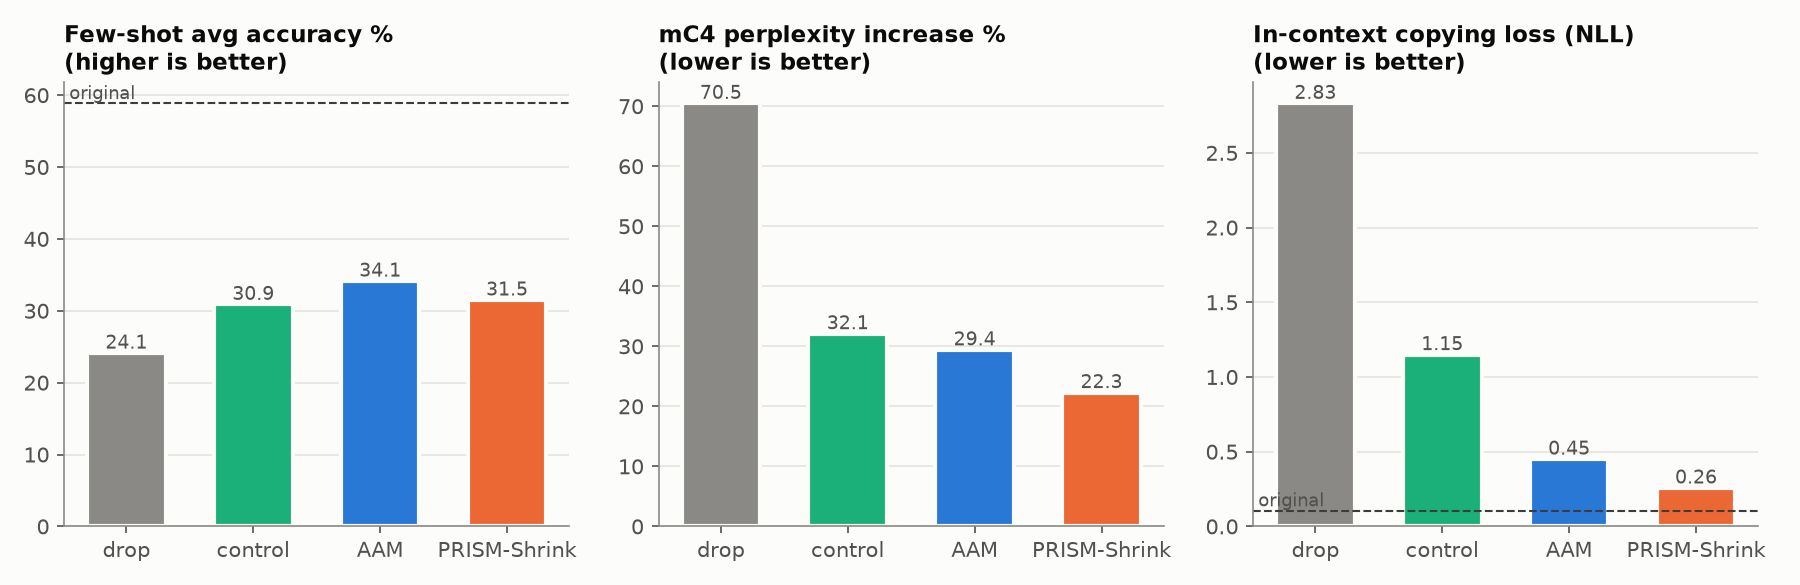
\includegraphics{model_17b.png}
\caption{Qwen3-1.7B-Base, 4 layers removed.}
\label{fig:17b}
\end{figure*}

\begin{figure}[t]
\centering
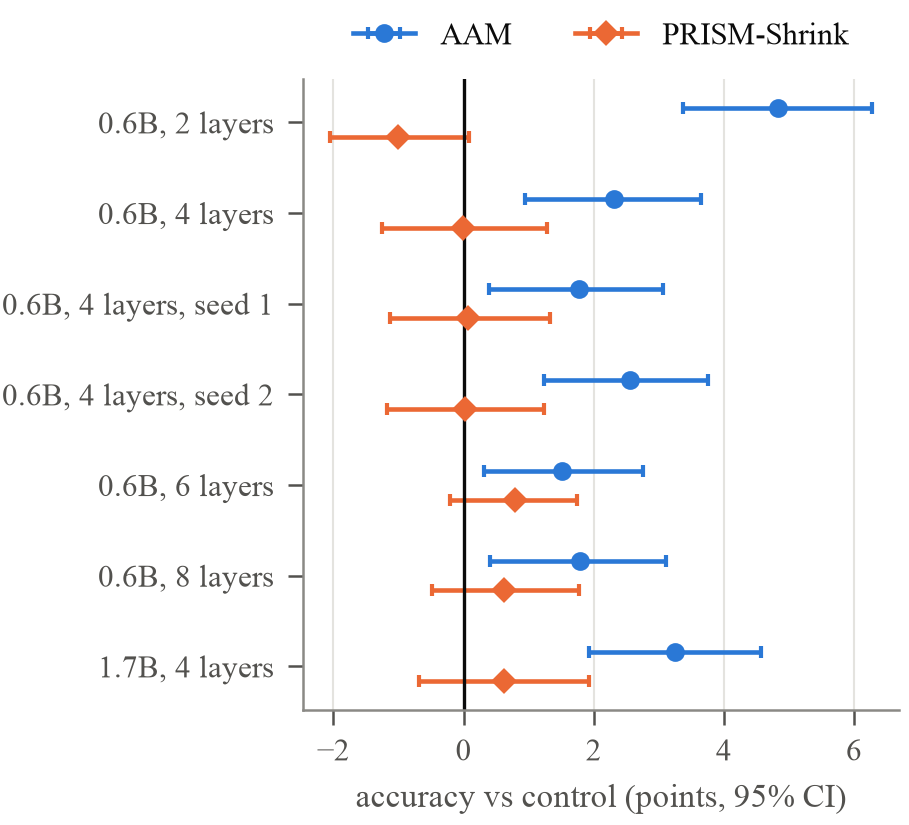
\includegraphics{diff_vs_control.png}
\caption{Accuracy difference to the matched control on the same questions (paired bootstrap, 95\%
CI). AAM is right of zero in every setting; PRISM-Shrink overlaps zero in every setting.}
\label{fig:forest}
\end{figure}

\begin{figure}[t]
\centering
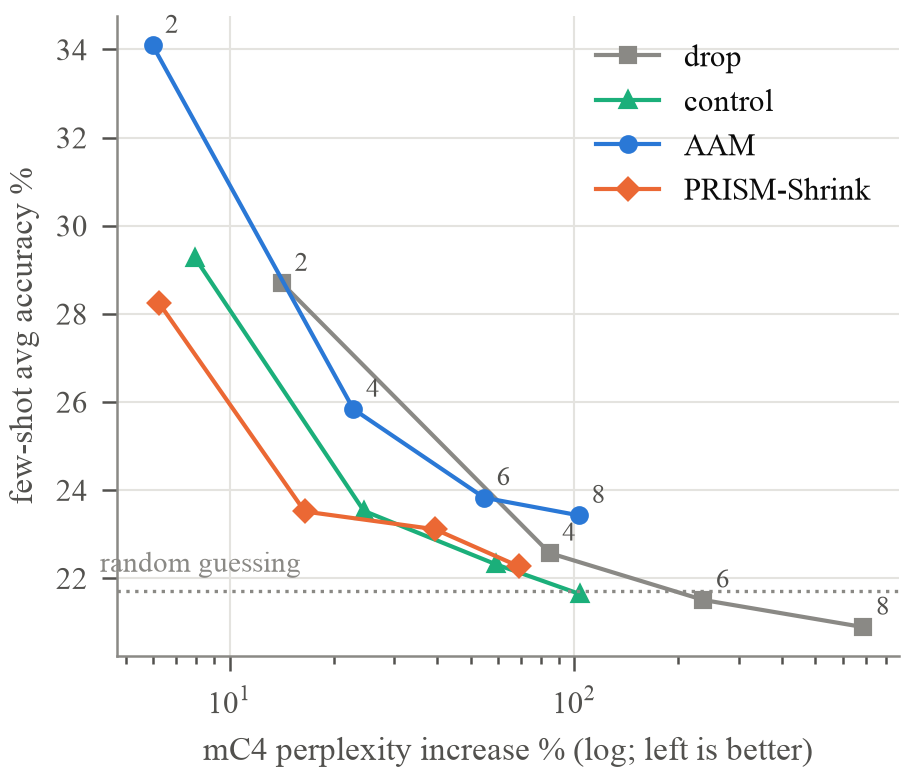
\includegraphics{tradeoff.png}
\caption{Accuracy against perplexity damage, Qwen3-0.6B; numbers are layers removed. AAM is highest, PRISM-Shrink is
furthest left.}
\label{fig:tradeoff}
\end{figure}

\begin{figure}[t]
\centering
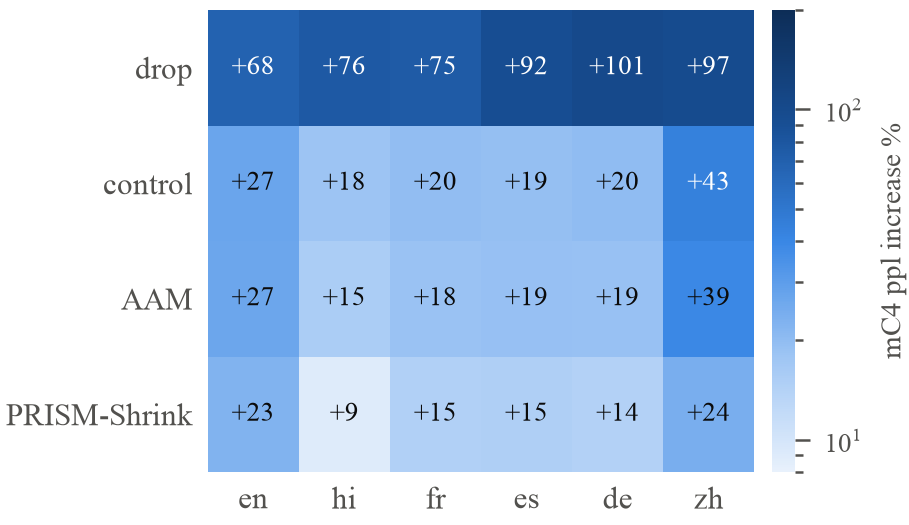
\includegraphics{per_language.png}
\caption{mC4 perplexity increase (\%) per language, Qwen3-0.6B, 4 layers removed. Chinese is hurt most;
PRISM-Shrink is lowest in every language.}
\label{fig:lang}
\end{figure}

\begin{figure}[t]
\centering
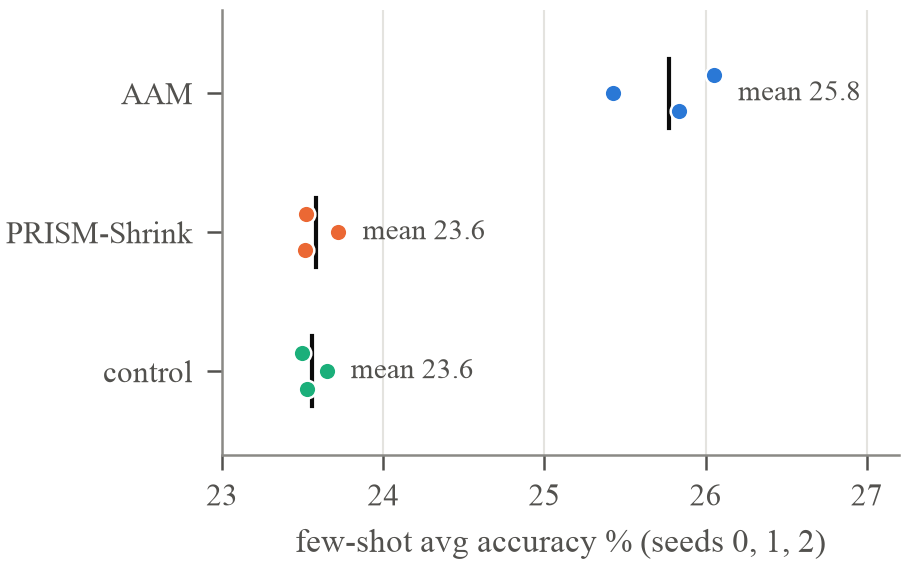
\includegraphics{seeds.png}
\caption{Three training seeds, Qwen3-0.6B, 4 layers removed; bars mark the means.}
\label{fig:seedsfig}
\end{figure}

\subsection{Deployment}

Every compressed model is a standard Qwen3 model with fewer layers, so it can be saved with
\texttt{save\_pretrained} and loaded with Hugging Face \texttt{transformers} without any custom code. I did not save
the trained models in these runs; the notebooks rebuild them. The research pipeline itself is already runnable: one
Kaggle notebook per experiment rebuilds the model, evaluates it and writes out the results
(Section~\ref{sec:impl}), and a 0.6B run takes about 1--1.5 hours on one T4. For inference the weights need about
1.2 GB (0.6B, fp16) or 3.4 GB (1.7B, fp16) of GPU memory. CPU inference works but is slow.

I chose an executable research pipeline over a web interface or API. The output of this project is a comparison of
methods, not a product, and every number has to be reproducible from code; a free Kaggle GPU also cannot host a
permanent service. End to end, the input is a model name, the layer count to remove and the method; the pipeline
picks the pairs, builds and distills the shortened model, evaluates it, and outputs one JSON row of results plus
the tables and figures. The same shortened model can be prompted directly with \texttt{generate} to show its text
output. Production deployment is not the goal: at 4 or more layers removed the 0.6B model is close to random
guessing, so it would not be useful to serve.

% =====================================================================================================================
\section*{Limitations}

With 4 or more layers removed from 0.6B, every method is close to random guessing and maths is lost entirely; this
is the main weakness of the work. PRISM-Shrink gives no accuracy gain, and its core idea has already been published
\citep{flattengpt}. Only the main 0.6B 4-layer runs have three seeds; every other setting is a single run. In the
main 0.6B comparison AAM was trained on plain text while the control and PRISM-Shrink were trained on ICL-packed
text. The text ablation puts this effect at 0.8 points at most, but the comparison is still not perfectly matched.

The study covers one model family, two small sizes, six languages and 200--250 questions per cell. Apart from MGSM
there are no instruction-following or generation-quality tests, and the hyperparameters were not tuned per method.
The quantization comparison comes from the literature rather than from my own test, and the speed numbers are noisy
because the GPUs were shared. Finally, some earlier experiments survive only as numbers, since their code and raw
results were never committed (see \texttt{docs/limitations\_and\_issues.md}).

% =====================================================================================================================
\section*{Team Contribution}

\begin{table}[h]
\centering\small
\resizebox{\columnwidth}{!}{%
\begin{tabular}{p{0.25\columnwidth}p{0.45\columnwidth}p{0.15\columnwidth}}
\toprule
Member & Contribution & Score \\
\midrule
Sumit Kumar Jha & data pipeline, methods, implementation, experiments, analysis, report & 100\,\% \\
\bottomrule
\end{tabular}}
\end{table}

\bibliography{custom}

% =====================================================================================================================
\appendix

\section{Additional results}

\begin{table}[h]
\centering\small
\resizebox{\columnwidth}{!}{%
\begin{tabular}{lrrrrr}
\toprule
Method & MMMLU & INCL. & MGSM & Bele. & XNLI \\
\midrule
chance & 25 & 25 & 0 & 25 & 33.3 \\
original & 47.9 & 43.6 & 41.2 & 63.1 & 48.9 \\
drop & 26.0 & 28.3 & 2.2 & 19.8 & 36.6 \\
control & 26.1 & 27.9 & 2.1 & 19.7 & 41.9 \\
AAM & 30.1 & 27.1 & 2.1 & 27.8 & 42.1 \\
PRISM-Shrink & 25.4 & 29.0 & 1.4 & 23.8 & 38.0 \\
\bottomrule
\end{tabular}}
\caption{Accuracy (\%) per benchmark, Qwen3-0.6B, 4 layers removed, mean of the six languages.}
\label{tab:bench}
\end{table}

\begin{table}[h]
\centering\small
\resizebox{\columnwidth}{!}{%
\begin{tabular}{lrrrr}
\toprule
Benchmark & ours 0.6B & official & ours 1.7B & official \\
\midrule
MMLU (en) & 54 & 52.8 & 59 & 62.6 \\
MMMLU & 47.9 & 50.2 & 50.9 & 63.3 \\
INCLUDE & 43.6 & 34.3 & 54.6 & 45.6 \\
MGSM & 41.2 & 31.0 & 58.8 & 50.7 \\
\bottomrule
\end{tabular}}
\caption{Original models on this test vs the Qwen3 report \citep{qwen3}, Table 8. Differences come from the
languages (6 here), question subsets, prompts and MGSM shots (4 vs 8).}
\label{tab:official}
\end{table}

\begin{table}[h]
\centering\small
\begin{tabular}{lrr}
\toprule
Language & Unique test tokens & Perplexity tokens \\
\midrule
en & 139{,}093 & 65{,}536 \\
hi & 330{,}752 & 65{,}536 \\
fr & 186{,}368 & 65{,}536 \\
es & 181{,}921 & 65{,}536 \\
de & 182{,}852 & 65{,}536 \\
zh & 156{,}288 & 65{,}536 \\
ja (unseen) & 197{,}929 & 65{,}536 \\
ru (unseen) & 168{,}363 & 65{,}536 \\
\bottomrule
\end{tabular}
\caption{Size of the large test per language (Qwen3-0.6B tokenizer).}
\label{tab:tokens}
\end{table}

\begin{table}[h]
\centering\small
\resizebox{\columnwidth}{!}{%
\begin{tabular}{llr}
\toprule
Session & Outcome & Hours \\
\midrule
reference (0.6B) & complete & 3.03 \\
data ablation & complete & 1.31 \\
deep methods & error (Shrink OOM) & 1.94 \\
reference (1.7B) & error (dtype) & 1.73 \\
deep control + Shrink plain & complete & 3.51 \\
reference (1.7B), re-run & complete & 0.77 \\
methods (1.7B) & error (Shrink OOM) & 1.12 \\
Shrink deep 6 / 8 & complete & 1.47 \\
Shrink + control (1.7B) & complete & 1.09 \\
1000 steps & complete & 1.27 \\
seeds AAM & complete & 1.05 \\
seeds Shrink & complete & 1.40 \\
seeds control & complete & 1.34 \\
\midrule
Total & & 21.0 \\
\bottomrule
\end{tabular}}
\caption{Logged Kaggle GPU sessions of the large-test queue (two T4 GPUs each). Failed sessions were fixed and re-run;
the AAM halves of the two out-of-memory sessions are used.}
\label{tab:gpu}
\end{table}

\begin{figure}[h]
\centering
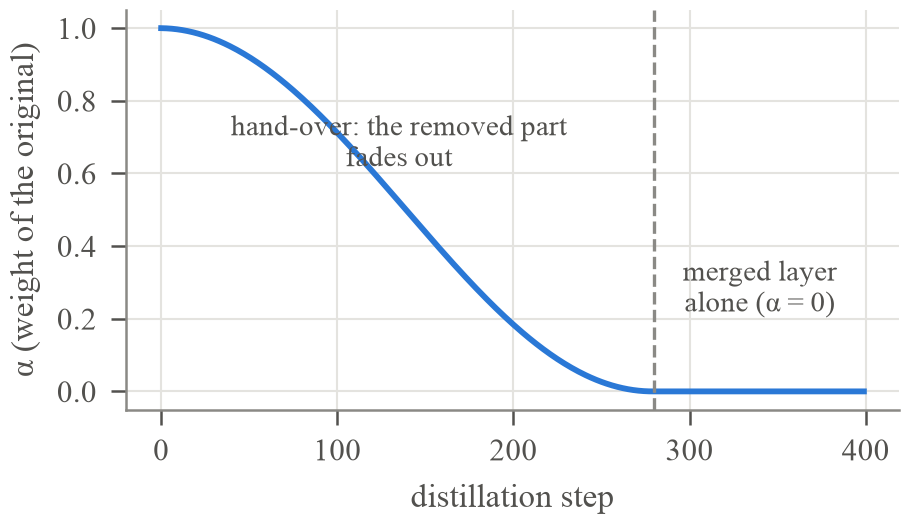
\includegraphics{alpha_schedule.png}
\caption{The fade schedule $\alpha$ over training steps.}
\label{fig:alpha}
\end{figure}

\begin{figure*}[t]
\centering
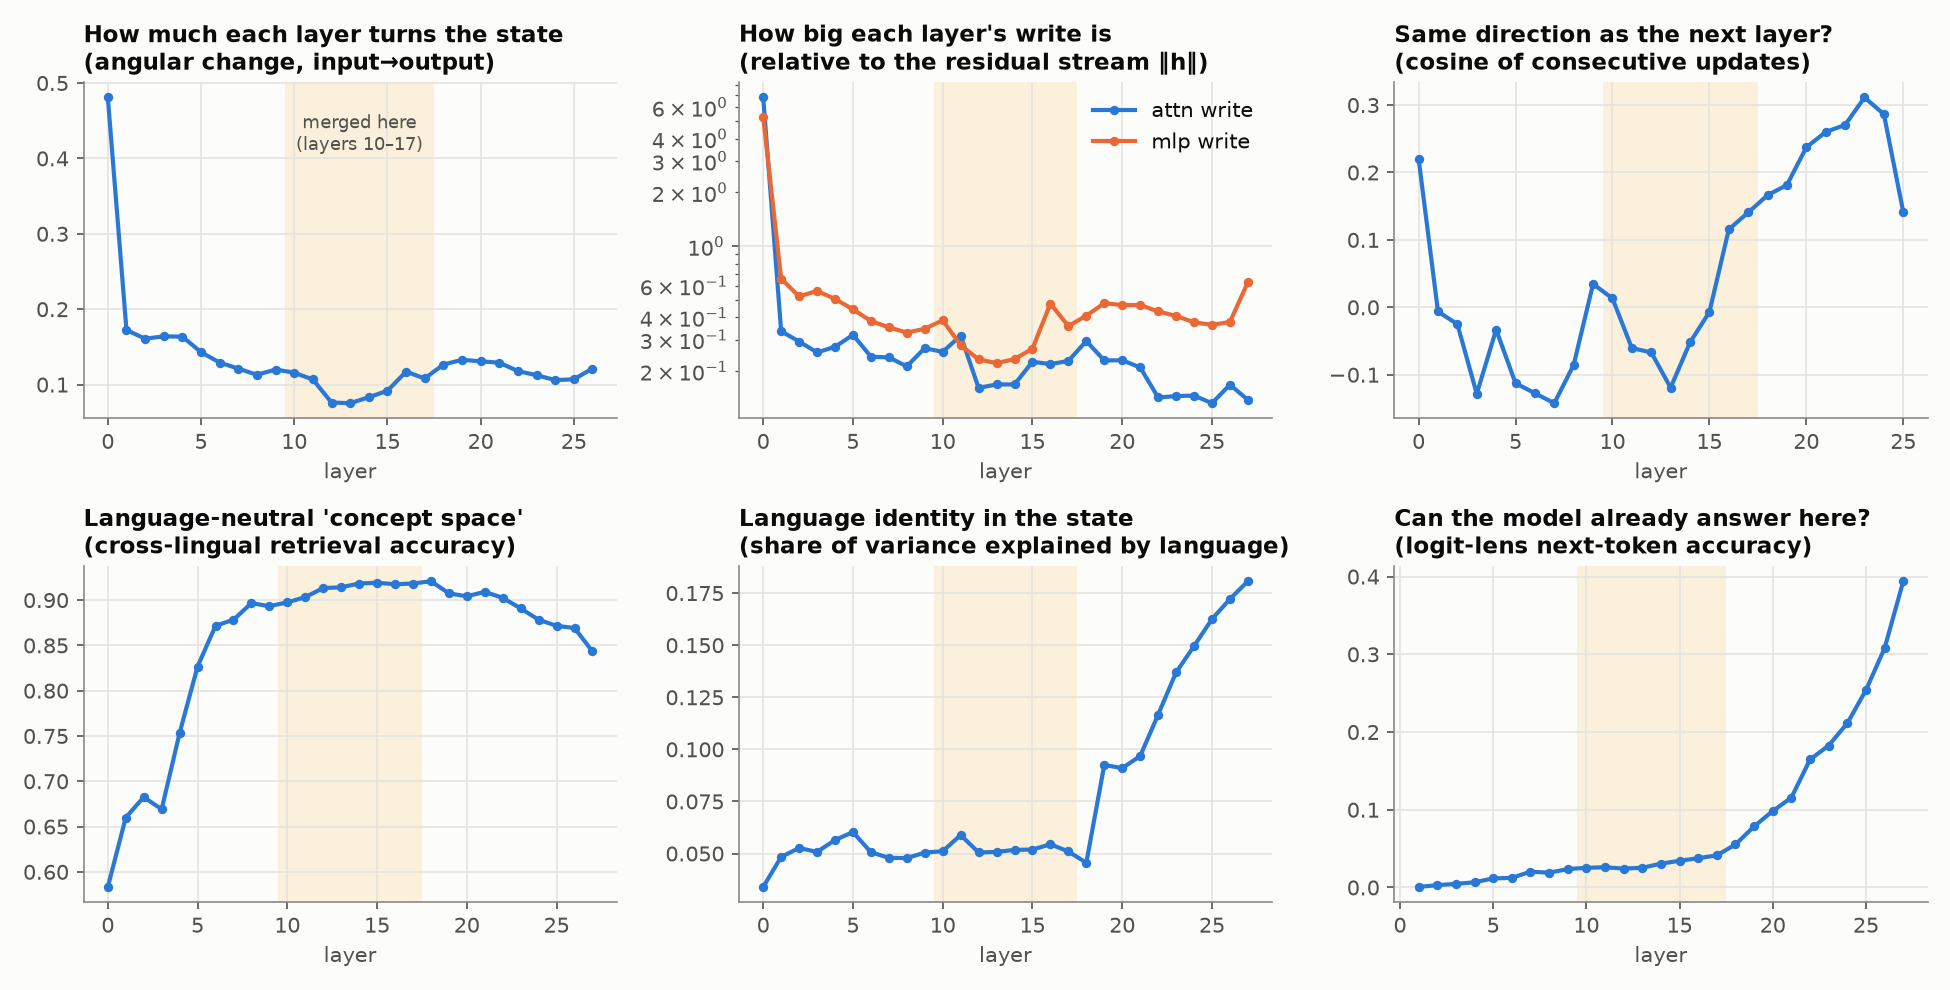
\includegraphics{layer_profile.png}
\caption{Layer analysis of Qwen3-0.6B (shaded: the layers merged at 4 layers removed). The middle layers change the
state least (a) and write least (b); language identity and next-token readiness grow only in the last third (e, f).}
\label{fig:layers}
\end{figure*}

\IfFileExists{screenshots/01_data.png}{\section{Screenshots of the pipeline}}{}

\shot{01_data.png}{Data preparation: Wiki-40B, mC4 and the five benchmarks downloaded and split.}
\shot{02_pairs.png}{Layer analysis: angular distance per layer and the chosen pairs.}
\shot{03_training.png}{Building the merged model and distillation (loss over steps).}
\shot{04_eval.png}{Evaluation: perplexity, benchmark accuracy and the copying probe.}
\shot{05_kaggle.png}{The Kaggle session queue (Table~\ref{tab:gpu}).}
\shot{06_analysis.png}{Rebuilding the tables and figures with \texttt{tools/analyze.py} and \texttt{make\_figures.py}.}

\end{document}
